\documentclass[11pt,a4paper,openany]{report}

\usepackage[T1]{fontenc}
\usepackage[utf8]{inputenc}
\usepackage{lmodern}
\usepackage{microtype}
\usepackage{amsmath,amssymb,amsthm,mathtools,bm}
\usepackage{booktabs,array,longtable,tabularx}
\usepackage{xcolor}
\usepackage[margin=24mm,headheight=23pt]{geometry}
\usepackage{enumitem}
\usepackage{fancyhdr}
\usepackage{fancyvrb}
\usepackage{graphicx}
\usepackage{url}
\usepackage{hyperref}

\definecolor{finblue}{HTML}{1F5A99}
\definecolor{fingreen}{HTML}{19733A}
\definecolor{finorange}{HTML}{D55E00}
\definecolor{finred}{HTML}{A61B1B}
\definecolor{finviolet}{HTML}{6A3D9A}
\definecolor{fingray}{HTML}{4D4D4D}

\hypersetup{
  unicode=true,
  colorlinks=true,
  linkcolor=finblue,
  citecolor=fingreen,
  urlcolor=finblue,
  pdftitle={FIN Post-41--50 Scientific Correction},
  pdfauthor={Krzysztof \.Zuchowski},
  pdfsubject={Methodology audit, mirror-coupling theorem, and canonical kernel policy},
  pdfkeywords={FIN, strict kernel, legacy kernel, mirror coupling, symmetry breaking, selector}
}

\pagestyle{fancy}
\fancyhf{}
\fancyhead[L]{\small FIN Post-41--50 Scientific Correction}
\fancyhead[R]{\small Release 10.5}
\fancyfoot[C]{\thepage}
\setlength{\parindent}{0pt}
\setlength{\parskip}{0.55em}
\setlist{nosep,leftmargin=2em}
\setcounter{tocdepth}{2}
\setcounter{secnumdepth}{3}
\emergencystretch=2em

\newcommand{\one}{\bm 1}
\newcommand{\C}{\mathbb C}
\newcommand{\R}{\mathbb R}
\newcommand{\Z}{\mathbb Z}
\newcommand{\statusProven}{\textcolor{fingreen}{[Proven]}}
\newcommand{\statusStrong}{\textcolor{finblue}{[Strong evidence]}}
\newcommand{\statusModerate}{\textcolor{finviolet}{[Moderate evidence]}}
\newcommand{\statusConditional}{\textcolor{finorange}{[Conditional]}}
\newcommand{\statusRefuted}{\textcolor{finred}{[Refuted]}}

\begin{document}
\hypersetup{pageanchor=false}
\begin{titlepage}
\centering
\vspace*{10mm}
{\Large\bfseries FIN Research Supplement --- Release 10.5\par}
\vspace{11mm}
{\Huge\bfseries FIN Post-41--50 Scientific Correction\par}
\vspace{6mm}
{\Large Methodology Audit, Mirror-Coupling Theorem, and Canonical Kernel Policy\par}
\vspace{17mm}
{\Large Krzysztof \.Zuchowski\par}
\vspace{2mm}
{\normalsize Independent Researcher --- Fractal Information Theory Project\par}
\vspace{2mm}
{\normalsize ORCID: \href{https://orcid.org/0009-0002-0909-3613}{0009-0002-0909-3613}\par}
\vspace{10mm}
{\large 27 July 2026\par}
{\normalsize Publication --- Preprint; record version 1.0.0\par}
\vfill
\begin{minipage}{0.88\textwidth}
\small
\textbf{Scope.} Scientific correction of the post-Programs-31--40 research,
including Programs 41--50 and P3172, followed by an executable mirror-coupling
audit and a canonical strict/legacy kernel policy.

\medskip
\textbf{Guardrail.} No silent legacy--strict identification, no role transfer,
no strict selector closure, no physical unit export, and no
Theory-of-Everything claim.

\medskip
\textbf{Reproducibility.}
\path{fin_post_41_50_correction_and_mirror.py},
\path{FIN_Post_41_50_Corrected_Results.json}, and the three generated figures.

\medskip
\textbf{License.} Creative Commons Attribution 4.0 International (CC BY 4.0).
\end{minipage}
\vfill
\end{titlepage}
\hypersetup{pageanchor=true}

\pagenumbering{roman}
\tableofcontents
\clearpage
\pagenumbering{arabic}

\section{Confidence convention}

\begin{itemize}
\item 
\textbf{\statusProven{}} analytic theorem or exact finite algebra under the stated definitions.

\item 
\textbf{\statusStrong{}} reproducible finite computation with a clear margin.

\item 
\textbf{\statusModerate{}} conclusion restricted to a declared model class.

\item 
\textbf{\statusConditional{}} valid only after an additional operator, state, clock, or sector axiom.

\item 
\textbf{\statusRefuted{}} contradicted by an explicit calculation or counterexample.

\end{itemize}

All quantities in this report are dimensionless. No SI unit, physical clock, strict selector, legacy-role transfer, completed legacy-to-strict bridge, unit-bearing action, or Theory-of-Everything claim is exported.

\par\medskip\hrule\medskip

\chapter{Executive summary}

This report re-audits the research artifacts added after Programs 31–40, including Program 42a, Programs 41–50, the legacy-star bridge audits, and P3171/\allowbreak{}P3172. It corrects methodological errors in the executable suite, performs new mirror-coupling tests, and freezes a kernel policy for subsequent work.

The principal conclusions are:

\begin{enumerate}
\item 
\textbf{There is no third canonical legacy kernel. \statusProven{}} The object called \[
   K^*(d)=A\frac{\cos(\pi d/4+\pi/6)}{1+\beta d}
   \] is a two-parameter family containing the already canonical legacy kernel exactly at \[
   A=4\ln2,\qquad \beta=0.01.
   \] The maximum difference is numerically zero.

\item 
\textbf{The freezes \((A,\beta)=(2.9,0.05)\) and \((1,1)\) are not canonical. \statusProven{}} Their relative profile distances from the canonical legacy object on \(d=1,\ldots,12\) are \(0.17892\) and \(0.94094\), respectively. They remain useful stress tests only.

\item 
\textbf{The P3172 Gram threshold is corrected. \statusProven{}} On the declared undirected \(Z_{12}\) Gram realization, \[
   \beta_*=1.075150776229914,
   \] not \(1.089\). The old value was the first positive point of an 80-point grid.

\item 
\textbf{The threshold is not universal. [Proven finite counterexamples]} Across cycle sizes \(N=8,10,12,14,16,20,24,32\), the threshold ranges from \(0.61472\) to \(1.11505\). It is a support-dependent finite property, not a physical constant.

\item 
\textbf{The raw quantity \(d_I=-\log|K|\) is not a metric. [Proven correction]} Previous code checked only the triangle inequality. The raw quantity has \[
   d_I(x,x)=-\log|A\cos(\pi/6)|,
   \] which is generally nonzero. At \(\beta=1\) the raw triangle inequality happens to hold on \(Z_{12}\), but the metric axioms still fail. Normalization by \(K(0)\) restores the zero diagonal but creates 96 triangle violations at \(\beta=1\). A genuine finite metric appears in the tested normalized construction only at the separate benchmark \(\beta=2\).

\item 
\textbf{The Program 42 phase fit is a tautology. [Proven correction]} Since both phases are affine in \(d\), \[
   \theta_s(d)=a\theta_\ell(d)+b,
   \quad
   a=\frac{\omega_s}{\omega_\ell},
   \quad
   b=\phi_s-a\phi_\ell,
   \] identically for every real \(d\). Its near-zero residual results from inserting the strict target parameters and has no predictive content.

\item 
\textbf{Program 43 contained data leakage. [Corrected]} Its declared training set was \(d=1,\ldots,4\), but the objective used all six points. The corrected training-only fit gives \[
   c=0.47447756,\qquad \eta=1.89178313,
   \] with training relative error \(0.137813\) and held-out \(d=5,6\) error \(0.999021\). The loss law does not generalize.

\item 
\textbf{The original Program 46 did not use its coupling operator. [Corrected]} It manually flipped an interference term after constructing an unused operator. The corrected test uses an actual mirror-odd Hermitian coupling.

\item 
\textbf{Mirror coupling has a precise but limited role. \statusProven{}} A passive reflected copy preserves symmetry. An inversion-odd carrier \(C\) with \(RCR=-C\) breaks reflection in a fixed branch \[
   H_\lambda=H_0+\lambda C,\qquad \lambda\ne0,
   \] but \[
   RH_\lambda R=H_{-\lambda}.
   \] The two branches are exactly isospectral. Thus \(C\) has the representation type required by the missing orientation object, but the sign/\allowbreak{}source law for \(\lambda\) is still absent.

\item 
\textbf{The kernel policy is now fixed.} Strict work uses \(K_{\rm strict\_gate}\). The only canonical non-strict bridge kernel is \(K_{\rm legacy\_ont}\) with \(A=4\ln2,\beta_{\rm tors}=0.01\). The legacy-star notation denotes an uncertainty family, not a new canonical kernel.

\end{enumerate}

\par\medskip\hrule\medskip

\chapter{Scope and repository guardrails}

The current repository distinguishes:

\[
K_{\rm legacy\_ont}(d)
=
4\ln2\,
\frac{\cos(\pi d/4+\pi/6)}{1+0.01d},
\]

an intermediate ontological/\allowbreak{}bridge kernel, from

\[
K_{\rm strict\_gate}(d)
=
\frac{\cos(0.18575d+0.16250)}{1+d^{1.8}},
\]

the later gate-selected strict working kernel.

This report treats strict as the primary strict object and legacy as an intermediate bridge object. It does not transfer legacy electroweak, electromagnetic, hierarchy, or torsion roles to strict.

The nadsoliton remains the primordial information in a solitonic state. No lower informational substrate is introduced.

\par\medskip\hrule\medskip

\chapter{Audit of the new research methodology}

\begin{center}
\begingroup\small
\setlength{\tabcolsep}{3.5pt}
\renewcommand{\arraystretch}{1.16}
\begin{longtable}{@{}p{0.244\textwidth}p{0.308\textwidth}p{0.308\textwidth}@{}}
\toprule
\textbf{Artifact or program} & \textbf{Original methodological status} & \textbf{Correction} \\
\midrule
\endhead
Program 42a reconstruction & Useful historical audit, but calls an already documented functional class a new reconstruction & Retain as conditional diagram audit; identify \(K^*\) as the parameter family containing canonical legacy \\
Program 41 Loewner scan & Finite support comparison & Keep only as support/\allowbreak{}normalization counterexample; not a universal bridge test \\
Program 42 phase map & Target-inserted affine fit & Reclassify as exact coordinate identity with zero predictive content \\
Program 43 hazard & Objective leaked held-out points & Restrict objective to \(d=1,\ldots,4\); held-out failure remains \\
Program 44 information flow & Correct after declared positivity repair & Retain; it compares temporal calculi, not physical time selection \\
Program 45 environment recovery & Chosen Stinespring dilation & Retain as an existence witness, not a kernel-derived bath or unique recovery mechanism \\
Program 46 sign reference & Coupling operator constructed but unused & Replace with \(H_\lambda=H_0+\lambda C\), \(RCR=-C\) \\
Program 47 influence proxy & Post-hoc two-parameter regression & Retain only as a failed phenomenological fit \\
Program 48 feedback & Open-spiral proxy called work & Replace with the closed unit-circle integral \(3.4\pi=10.6814\) \\
Program 49 process tensor & Comparison of two Markov semigroups & Relabel as two-generator intervention discrimination, not a full process-tensor test \\
Program 50 challenge & Strict-generated target scored against strict & Reclassify as software self-recovery; no independent evidence \\
P3172 metric & Checked triangle inequality only & Check zero diagonal, nonnegativity, separation, symmetry, and triangle inequality \\
P3172 PSD threshold & First passing point on coarse grid & Bracket and bisect the eigenvalue crossing \\
\bottomrule
\end{longtable}
\endgroup
\end{center}

The corrected Programs 41–50 executable and JSON were regenerated.

\par\medskip\hrule\medskip

\chapter{Corrected finite results}

\section{Legacy-star is a family, not a third kernel}

Define

\[
\mathcal K_*=
\left\{
A\frac{\cos(\pi d/4+\pi/6)}{1+\beta d}
:
A>0,\ \beta>0
\right\}.
\]

Then

\[
K_{\rm legacy\_ont}\in\mathcal K_*
\]

exactly at \(A=4\ln2\), \(\beta=0.01\). Therefore the terminology should be:

\begin{itemize}
\item 
K\_legacy\_ont: canonical legacy bridge kernel;

\item 
LegacyStarRadialFamily: parameter family for uncertainty and stress testing;

\item 
not K\_legacy\_star as a separate canonical physical kernel.

\end{itemize}

\begin{figure}[htbp]
\centering
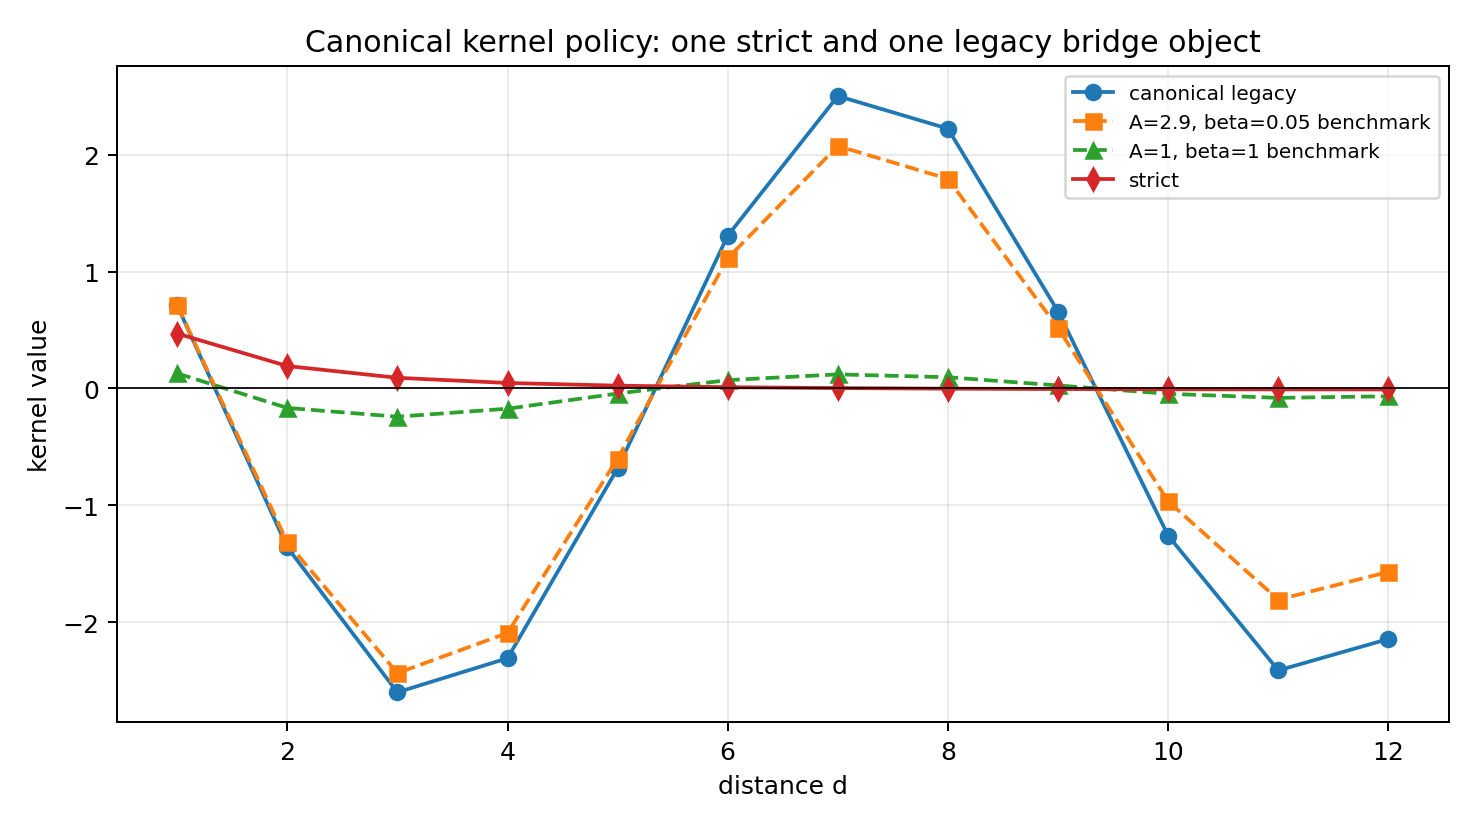
\includegraphics[width=0.92\textwidth]{FIN_Post_41_50_Correction_Figures/kernel_policy_profiles.png}
\caption{Canonical strict and legacy profiles together with the two noncanonical legacy-family benchmark freezes.}
\end{figure}


\section{Gram positivity is support dependent}

The exact finite thresholds are:

\begin{center}
\begingroup\small
\setlength{\tabcolsep}{3.5pt}
\renewcommand{\arraystretch}{1.16}
\begin{longtable}{@{}p{0.420\textwidth}p{0.420\textwidth}@{}}
\toprule
\textbf{Cycle size \(N\)} & \textbf{\(\beta_*(N)\)} \\
\midrule
\endhead
8 & 0.806516886 \\
10 & 1.115047101 \\
12 & 1.075150776 \\
14 & 0.795468336 \\
16 & 0.614721534 \\
20 & 0.858165892 \\
24 & 0.729453278 \\
32 & 0.676222037 \\
\bottomrule
\end{longtable}
\endgroup
\end{center}

\begin{figure}[htbp]
\centering
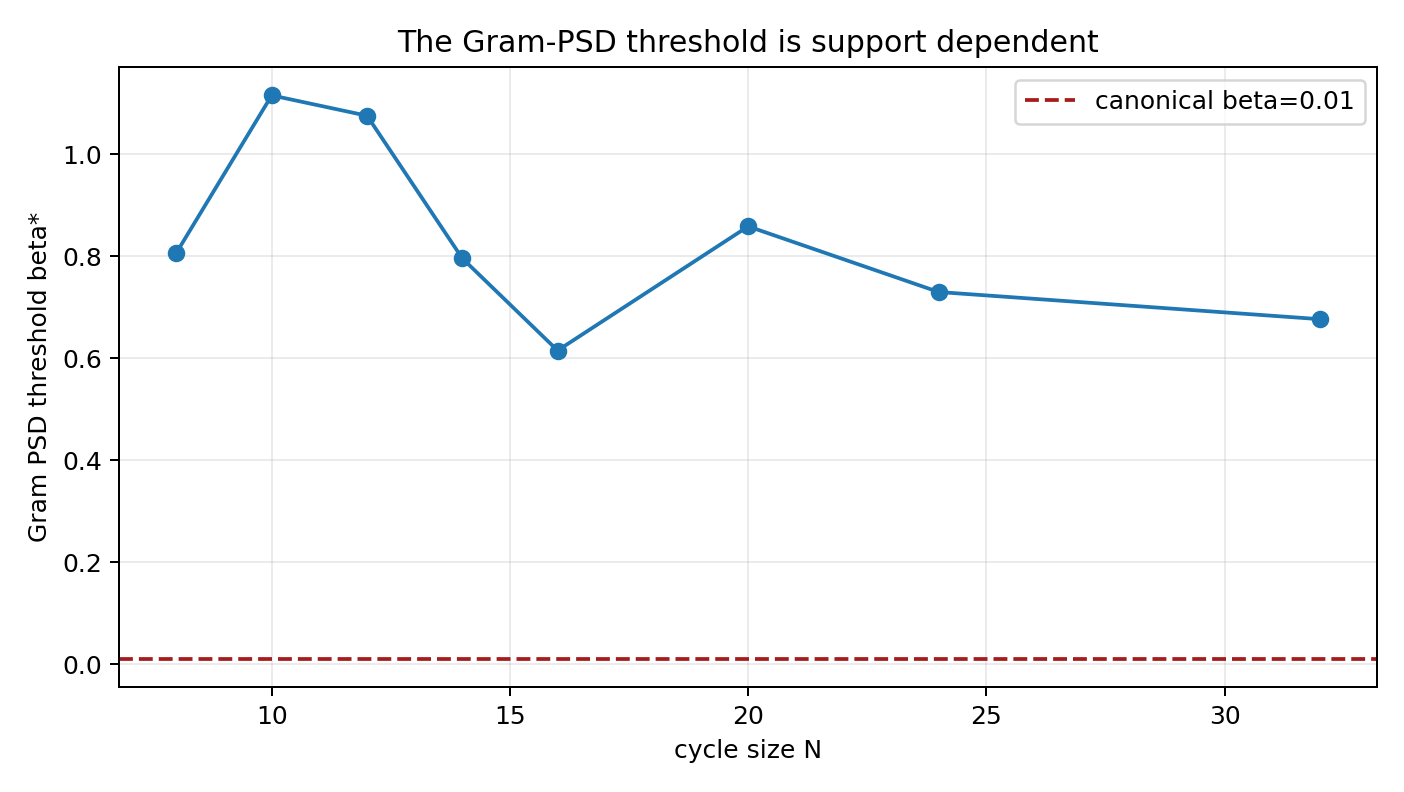
\includegraphics[width=0.92\textwidth]{FIN_Post_41_50_Correction_Figures/psd_threshold_support_scan.png}
\caption{The Gram-positive threshold depends on the finite cycle support; it is not a universal constant.}
\end{figure}


The canonical \(\beta_{\rm tors}=0.01\) is far below every listed Gram threshold. This does not invalidate the signed kernel as a self-adjoint interaction operator. It does invalidate interpreting its undirected matrix as a covariance/\allowbreak{}Gram kernel without an additional transformation.

\section{Information-distance correction}

For raw

\[
d_I(x,y)=-\log|K(d(x,y))|,
\]

the diagonal is not zero. Therefore it is not a metric at \(\beta=0.01,1,\) or \(2\), even when the triangle inequality happens to hold.

For the normalized candidate

\[
\widetilde d_I(x,y)
=
-\log\frac{|K(d(x,y))|}{|K(0)|},
\]

the finite results are:

\begin{center}
\begingroup\small
\setlength{\tabcolsep}{3.5pt}
\renewcommand{\arraystretch}{1.16}
\begin{longtable}{@{}p{0.090\textwidth}p{0.269\textwidth}p{0.250\textwidth}p{0.251\textwidth}@{}}
\toprule
\textbf{\(\beta\)} & \textbf{Nonnegative?} & \textbf{Triangle violations} & \textbf{Metric on tested \(Z_{12}\)?} \\
\midrule
\endhead
0.01 & no & 216 & no \\
1 & yes & 96 & no \\
2 & yes & 0 & yes \\
\bottomrule
\end{longtable}
\endgroup
\end{center}

This is a finite regime statement, not a canonical geometry theorem.

\section{Corrected hazard generalization}

The corrected fit uses only distances \(1\)–\(4\). The held-out error is approximately one:

\[
\varepsilon_{\rm train}=0.137813,
\qquad
\varepsilon_{\rm hold}=0.999021.
\]

The apparent exponent near \(1.9\) is not a derivation of strict \(\eta=1.8\); it is an unstable target-conditioned fit.

\section{Feedback correction}

For

\[
M=
\begin{pmatrix}
-0.8&-1.7\\
1.7&-0.8
\end{pmatrix},
\]

the eigenvalues are \(-0.8\pm1.7i\). The full normalized antisymmetry defect is

\[
\frac{\|M-M^T\|_F}{\|M\|_F}=1.8096374.
\]

The genuine unit-circle work is

\[
\oint_{|z|=1}(Mz)\cdot dz
=
3.4\pi
=
10.6814150.
\]

Stable feedback therefore need not be a gradient flow. This feedback law remains added rather than kernel-derived.

\par\medskip\hrule\medskip

\chapter{Mirror-coupling theorem}

\section{Passive reflection does not break symmetry}

Let \(R\) be the reflection operator on \(Z_{12}\), \(R^2=I\). The canonical radial legacy matrix \(H_0\) satisfies

\[
RH_0R=H_0
\]

with zero finite residual.

Consequently:

\begin{itemize}
\item 
replacing \(H_0\) by \(RH_0R\) changes nothing;

\item 
coupling \(H_0\) to an identical reflected copy with a symmetric off-diagonal block preserves a \(Z_2\) sector-exchange symmetry;

\item 
the sign of an isolated two-copy coupling \(g\) is a gauge, because a sign flip on one copy maps \(g\) to \(-g\).

\end{itemize}

The finite two-copy sign-gauge and mirror-commutator residuals are both zero.

\section{The inversion-odd carrier}

Choose a directed representative \(D\) of the legacy-star family and define

\[
C
=
\frac{i}{2}(D-D^T).
\]

Then \(C=C^\dagger\) and

\[
RCR=-C.
\]

After Frobenius normalization, define

\[
H_\lambda=H_0+\lambda C.
\]

For \(\lambda=0.4\), the finite tests give:

\begin{center}
\begingroup\small
\setlength{\tabcolsep}{3.5pt}
\renewcommand{\arraystretch}{1.16}
\begin{longtable}{@{}p{0.420\textwidth}p{0.420\textwidth}@{}}
\toprule
\textbf{Test} & \textbf{Residual or value} \\
\midrule
\endhead
\(RH_0R-H_0\) & 0 \\
\(RCR+C\) & 0 \\
\(RH_{+\lambda}R-H_{-\lambda}\) & 0 \\
spectral difference \(H_{+\lambda}\) vs \(H_{-\lambda}\) & 0 \\
fixed-branch reflection commutator norm & 0.8 \\
\bottomrule
\end{longtable}
\endgroup
\end{center}

Thus:

\begin{quote}\itshape
\textbf{Mirror theorem.} A nonzero inversion-odd coupling explicitly breaks reflection in a fixed signed branch, but the full \(+\lambda/-\lambda\) pair remains reflection symmetric and isospectral.

\end{quote}

This theorem separates three claims:

\begin{enumerate}
\item 
existence of an odd carrier \(C\): \textbf{constructed};

\item 
breaking of reflection after fixing \(\lambda\ne0\): \textbf{proven};

\item 
internal selection of the sign of \(\lambda\): \textbf{not obtained}.

\end{enumerate}

\section{Does it match a missing theoretical object?}

Yes, partially.

The operator \(C\) has exactly the inversion-odd/\allowbreak{}chiral representation type identified in the selector and orientation audits. It is a candidate carrier for:

\begin{itemize}
\item 
the orientation torsor;

\item 
a chiral or pseudoscalar sector;

\item 
a signed current;

\item 
a polarity-sensitive apparatus coupling.

\end{itemize}

However, the construction of \(D\) already chooses a directed chart, and the scalar legacy kernel does not supply:

\begin{itemize}
\item 
a nonzero signed value of \(\lambda\);

\item 
a law choosing \(+\lambda\) rather than \(-\lambda\);

\item 
a coupling theorem from the informational nadsoliton to \(C\);

\item 
a phase origin;

\item 
a physical scale.

\end{itemize}

Therefore mirror coupling provides the \textbf{receiver/\allowbreak{}representation object}, not the missing \textbf{source/\allowbreak{}selector theorem}.

\section{Classical directional realization}

A positive-rate directional model can be constructed as

\[
w_{i,i+r}(\lambda)=a_r e^\lambda,
\qquad
w_{i,i-r}(\lambda)=a_r e^{-\lambda},
\]

with \(a_r=|K_{\rm legacy}(r)|\). At \(\lambda=0.4\):

\begin{center}
\begingroup\small
\setlength{\tabcolsep}{3.5pt}
\renewcommand{\arraystretch}{1.16}
\begin{longtable}{@{}p{0.420\textwidth}p{0.420\textwidth}@{}}
\toprule
\textbf{Quantity} & \textbf{Value} \\
\midrule
\endhead
uniform stationary residual & \(6.0\times10^{-16}\) \\
mirror covariance residual & \(9.4\times10^{-15}\) \\
nearest-edge stationary current & 0.0486395 \\
entropy-production rate & 5.03545 \\
\bottomrule
\end{longtable}
\endgroup
\end{center}

The current is odd in \(\lambda\), while entropy production is even. Negative and positive couplings are mirror descriptions unless an external orientation reference fixes the sign.

\begin{figure}[htbp]
\centering
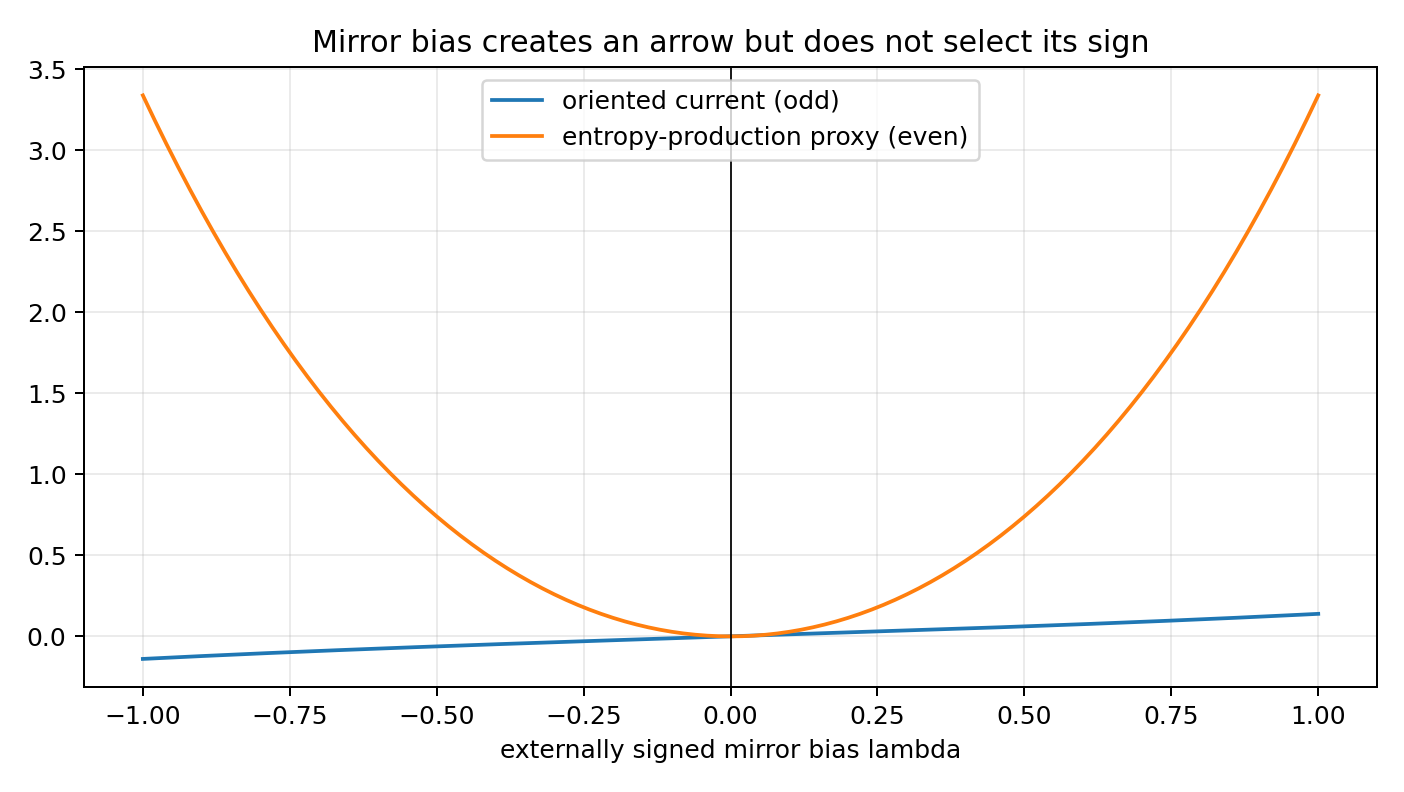
\includegraphics[width=0.92\textwidth]{FIN_Post_41_50_Correction_Figures/mirror_bias_current_entropy.png}
\caption{Directional current is odd in the mirror-bias parameter, whereas entropy production is even.}
\end{figure}


\par\medskip\hrule\medskip

\chapter{Canonical kernel policy for future work}

\section{Primary kernel}

Use

\[
K_{\rm strict\_gate}(d)
=
\frac{\cos(0.18575d+0.16250)}{1+d^{1.8}}
\]

for strict-pipeline calculations, strict dual dynamics, and any work claiming compatibility with the current strict gate.

\section{Only canonical kernel outside strict}

Use

\[
\boxed{
K_{\rm legacy\_ont}(d)
=
4\ln2\,
\frac{\cos(\pi d/4+\pi/6)}{1+0.01d}
}
\]

as the sole canonical non-strict intermediate bridge kernel.

\section{Objects that are not additional canonical kernels}

\begin{center}
\begingroup\small
\setlength{\tabcolsep}{3.5pt}
\renewcommand{\arraystretch}{1.16}
\begin{longtable}{@{}p{0.420\textwidth}p{0.420\textwidth}@{}}
\toprule
\textbf{Object} & \textbf{Future status} \\
\midrule
\endhead
\(K^*(A,\beta)\) & uncertainty/\allowbreak{}stress-test family containing canonical legacy \\
\(K^*(2.9,0.05)\) & historical diagram benchmark only \\
\(K^*(1,1)\) & finite operator-scale benchmark only \\
rejected double-damped product & retire \\
\(|K_{\rm legacy}|\) & declared magnitude projection for sensitivity tests, not a kernel identity \\
\(\max(K_{\rm legacy},0)\) & declared positive-part projection for sensitivity tests \\
mirror-odd \(C\) & conditional sector operator; not a replacement kernel \\
\bottomrule
\end{longtable}
\endgroup
\end{center}

\section{Dynamics policy}

\begin{itemize}
\item 
For primary Markov/\allowbreak{}diffusive work, use strict because its declared \(C_{12}\) weights are positive.

\item 
For legacy spectral/\allowbreak{}unitary work, use the signed self-adjoint legacy matrix; a scalar spectral shift may be used but must be declared.

\item 
For legacy Markov sensitivity, report both positive-part and absolute-value repairs. Programs 31–40 proved that the repair is nonunique and dynamically consequential.

\item 
Do not call either repair “the legacy kernel.”

\item 
Add \(C\) only in an explicitly conditioned sector-axiom branch.

\end{itemize}

\par\medskip\hrule\medskip

\chapter{What survives after correction}

\section{Proven or retained}

\begin{itemize}
\item 
Canonical legacy and strict remain distinct but related research objects.

\item 
The legacy-star functional family is mathematically useful.

\item 
Dual Borel dynamics from one self-adjoint generator remains valid.

\item 
Apparent reduced information loss remains compatible with environmental transfer.

\item 
The raw signed legacy kernel is not a classical Markov-rate matrix.

\item 
Mirror-odd coupling can create a genuine directional branch.

\item 
The \(+\lambda\) and \(-\lambda\) branches remain mirror-paired and isospectral.

\end{itemize}

\section{Refuted or demoted}

\begin{itemize}
\item 
A new third canonical legacy-star kernel.

\item 
Phase-fit residual as evidence of strict-phase derivation.

\item 
Program 50 as independent validation of strict.

\item 
Original Program 46 as an executed coupling test.

\item 
Raw \(-\log|K|\) as a metric merely because triangles pass.

\item 
\(\beta_*\) as a universal constant.

\item 
Mirror copying alone as symmetry breaking.

\item 
Mirror-odd carrier existence as selector closure.

\end{itemize}

\par\medskip\hrule\medskip

\chapter{Recommended continuation}

\begin{enumerate}
\item 
\textbf{Freeze the kernel policy in documentation.} Use only strict plus canonical legacy; treat all other freezes as benchmarks.

\item 
\textbf{Develop the mirror carrier only as a conditioned sector object.} Write \[
   H_{\lambda}=H_0+\lambda C
   \] with explicit SA\_mirror(lambda, orientation) labeling.

\item 
\textbf{Attack the real missing theorem:} derive or rule out a non-premise signed source law \[
   \mathrm{Source}_{\rm mirror}(\text{nadsoliton})\longrightarrow
   \lambda C,
   \qquad \lambda\ne0.
   \]

\item 
\textbf{Do not perform further scalar or affine phase fits.} They cannot source orientation or strict phase parameters.

\item 
\textbf{Replace synthetic self-recovery with blinded external targets.} A valid kernel-selection challenge must hide the generating model and must not include exact target code as a candidate by construction.

\item 
\textbf{Keep unit and selector frontiers separate.} Mirror chirality cannot supply \(S_+\), \(\hbar_*\), length, time, or action units.

\item 
\textbf{Run both quantum and stochastic mirror branches.} Test whether one signed \(\lambda\) explains orientation-sensitive records across both categories after clock and apparatus marginalization.

\end{enumerate}

\par\medskip\hrule\medskip

\chapter{Final scientific judgment}

The post-31–40 research contains useful finite mathematics, but several headline results were stronger than their methods justified. After correction, the scientifically stable structure is:

\[
\boxed{\begin{gathered}
K_{\rm legacy\_ont}\quad\text{(canonical intermediate bridge object)},\\
K_{\rm strict\_gate}\quad\text{(primary strict working object)}.
\end{gathered}}
\]

The legacy-star notation is retained only for the parameter family containing the canonical legacy kernel.

Mirror coupling does not solve the theory by passive reflection. Its nontrivial contribution is sharper:

\begin{center}
\fbox{\parbox{0.86\textwidth}{\centering It constructs the correct inversion-odd carrier, but not the law selecting its sign.}}
\end{center}

It therefore matches the shape of a missing theoretical object while leaving the actual selector, source provenance, dimensional scale, and legacy-to-strict bridge open.

\par\medskip\hrule\medskip

\chapter{Reproducibility}

\begin{itemize}
\item 
Corrected Programs 41–50 code: \path{fin_programs_41_50_legacy_star.py}

\item 
Corrected Programs 41–50 record: \path{FIN_Programs_41_50_Legacy_Star_Results.json}

\item 
P3172 corrected code and tests: \path{fundamental_action_reconstruction/p3172_s2122_legacy_star_operator_model_generator_potential_audit.py}

\item 
New correction/\allowbreak{}mirror suite: \path{fin_post_41_50_correction_and_mirror.py}

\item 
New machine-readable record: \path{FIN_Post_41_50_Corrected_Results.json}

\item 
Figures: \path{FIN_Post_41_50_Correction_Figures/}

\end{itemize}

Suggested citation:

Żuchowski, K. (2026). \emph{FIN Post-41–50 Scientific Correction: Methodology Audit, Mirror-Coupling Theorem, and Canonical Kernel Policy} (FIN Research Supplement, Release 10.5; Version 1.0.0) [Preprint].


\clearpage
\chapter*{Archival note}
\addcontentsline{toc}{chapter}{Archival note}
The numerical record \path{FIN_Post_41_50_Corrected_Results.json} is generated
by \path{fin_post_41_50_correction_and_mirror.py}. Corrected Programs 41--50 are
recorded by \path{fin_programs_41_50_legacy_star.py}. The exact P3172 threshold
and full metric-axiom audit are independently covered by its updated tests.

\medskip
\noindent\textbf{Suggested citation:}

\.Zuchowski, K. (2026). \emph{FIN Post-41--50 Scientific Correction:
Methodology Audit, Mirror-Coupling Theorem, and Canonical Kernel Policy}
(FIN Research Supplement, Release 10.5; Version 1.0.0) [Preprint].

\end{document}
